\documentclass[12pt]{article}
\usepackage{amsmath,amssymb,amsthm}
\usepackage{graphicx,mathabx}
\usepackage{xcolor}
\usepackage{tikz}
\usepackage{placeins}
\usepackage{lipsum}
\usepackage[shortlabels]{enumitem}
\usepackage{placeins}
\newcommand\tab[1][1cm]{\hspace*{#1}}
\begin{document}
\title{TCSS 343 - Week 4}
\author{Jake McKenzie}
\maketitle
\noindent\centerline{\textbf{Dynamic Programming}}\\\\\\\\\\\\\\\\
\begin{center}
    ``An optimal policy has the property that whatever the initial state and initial decision are, the remaining decisions must constitute an optimal policy with regard to the state resulting from the first decision." \\$\cdots$\\  Richard Bellman's \textbf{Principle of Optimality}
\end{center}
\begin{center}
    ``What we choose means more than what was handed to us by chance." \\$\cdots$\\  Ada Palmer
\end{center}
\begin{center}
    `` If `dynamic programming' didn't have such a cool name, it would be known as 'populating a table'". \\$\cdots$\\ Mark Dominus 
\end{center}
\newpage
\noindent 1. Today we're going to explore dynamic programming. Below are three implementations of the fibonacci algorithm that I wrote in python. I want you to draw the \textbf{``tree"} for each then reflect on how the ``bottom up" apprach is different from the other two? (Hint: They are all trees but also different types of trees. This is a key insight in my opinion in idea in understanding dynamic programming) \\
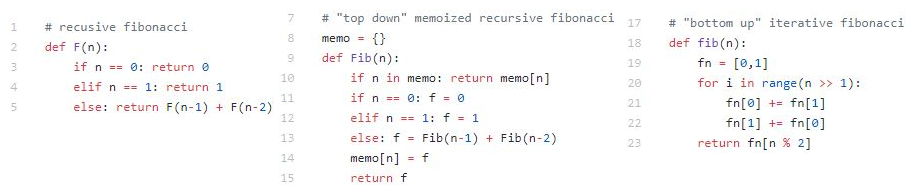
\includegraphics[width=\linewidth]{fib.jpg}
\newpage
\noindent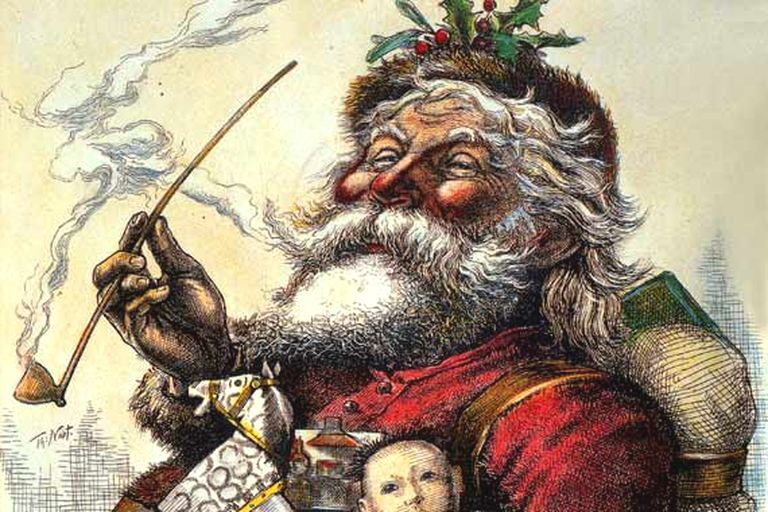
\includegraphics[scale = .3]{santa.jpg}\\
\noindent 2. Suppose Santa has 6 kinds of toys, each kind of toy has its own weight $w_i$ in tons, happiness rating $h_i$ in ... joy, and quantity $n_i$. Santa would like to maximize the total hapiness of the children but the total weight of his bag cannot exceed 17 tons. Their weight, hapiness rating and quantity are defined above. Please help Santa by filling in the DP table below, where dp[i][j] indicates the maximum value you can get with weight less or equal to $j$ using toys 1 to $i$. What is the final solution to this problem and briefly explain how you came to this solution. To help you get started, $23$ was generated by solving the equation $i_1+2i_2+3i_3 \leq 15$ which gives you the most value. That value was found by $3\cdot 1+ 2 \cdot 4 + 2 \cdot 6 = 23$. $12$ was found by solving the equation $i_1+2i_2+3i_3+4i_4+5i_5+6i_6 \leq 6$ which gives you the most value. That value was found by $2\cdot 6 = 12$ 
\begin{table}[]
\begin{tabular}{|l|l|l|l|}
\hline
i & $w_i$ & $h_i$ & $n_i$ \\ \hline
1 & 1    & 1    & 3    \\ \hline
2 & 2    & 4    & 2    \\ \hline
3 & 3    & 6    & 2    \\ \hline
4 & 4    & 5    & 1    \\ \hline
5 & 5    & 7    & 1    \\ \hline
6 & 6    & 8    & 1    \\ \hline
\end{tabular}
\end{table}
\FloatBarrier
\begin{table}[]
    \begin{tabular}{|l|l|l|l|l|l|l|l|l|l|l|l|l|l|l|l|l|l|l|}
    \hline
    i\textbackslash{}w & 0 & 1 & 2 & 3 & 4 & 5 & 6  & 7 & 8 & 9 & 10 & 11 & 12 & 13 & 14 & 15 & 16 & 17 \\ \hline
    1                  & 0 &   &   &   &   &   &    &   &   &   &    &    &    &    &    &    &    &    \\ \hline
    2                  & 0 &   &   &   &   &   &    &   &   &   &    &    &    &    &    &    &    &    \\ \hline
    3                  & 0 &   &   &   &   &   &    &   &   &   &    &    &    &    &    & 23 &    &    \\ \hline
    4                  & 0 &   &   &   &   &   &    &   &   &   &    &    &    &    &    &    &    &    \\ \hline
    5                  & 0 &   &   &   &   &   &    &   &   &   &    &    &    &    &    &    &    &    \\ \hline
    6                  & 0 &   &   &   &   &   & 12 &   &   &   &    &    &    &    &    &    &    &    \\ \hline
    \end{tabular}
    \end{table}
    \FloatBarrier
\newpage
\centerline{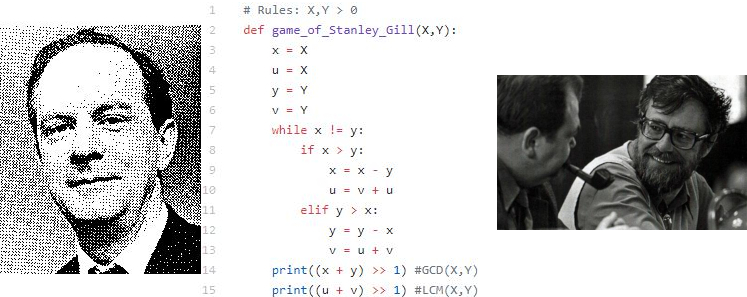
\includegraphics[scale = 2]{comb.jpg}}
\noindent 3. This is a game shown to Edsgar Dijkstra(pictured right) when he was still an undergraduate, attributed to Stanley Gill(pictured left), an early computer scientist. Now it is true that $2XY = xv+yu$, which can be seen when the variables are initialized. But it is always true given that $X,Y > 0$? Show why this is true. (Hint: You can use the comments to help you along. Remember that the $>> 1 $ operation is the same as $ / 2$.)
\newpage
\noindent 4. Hopefully in problem 1 I was able to impart on you the reality that most dynamic 
programming problems can be thought of as graph problems, specifically directed acyclic graphs, 
DAG for short. Even if you don't solve them with DAGs I think it's a useful headspace for a large class of problems. 
We can typically solve DP problems without constructing a graph. If we aren't going to use a graph there are other useful
tools that you may not have run across. Let's try to understand what a bitmask is. I've been peppering
them into the packets all quarter but let's finally dive deep into them. Mask in bitmask means hiding 
something. Bitmask is nothing but a binary number that represents something.\\\\
Please connect the corresponding ``bitmask" with their
set operations or arithmetic operations. I encourage you to 
play around with the operation and really try understand what
they're doing. All operations are on two intergers $X$ and $Y$. 
I know this may seem disjointed from what you've covered in
class but I have used all of these in solving DP problems. 
Often times we aren't just worried about our time complexity,
but we're also worried about space complexity. Using integers
instead of arrays to represent data is sometimes vital in solving
hard problems. For example: we may represent the set $\{5,4,3,2,1\}$ 
as $11111$ in binary which is $31$ in decimal and the set $\{4,2,1\}$ 
as $01011$ in binary which is $11$ in decimal.
\begin{enumerate}[a)]
    \item  $X \& 1 \tab\tab\tab$ I)Union of two sets
    \item  $X \wedge Y \tab\tab\tab$ II)Arithmetic negation
    \item  $ (X >> 31) \& 1 \tab\tab$ III)Test for set membership
    \item  $X | Y \tab\tab\tab\tab$IV)2 to the power of X(also Singleton Set)
    \item  $X \& Y \tab\tab\tab\tab$V)Barrel shift left
    \item  $X \&= (X - 1) \tab\tab\tab$VI)Intersection of two sets
    \item  $(X<<Y) | (X >> (32 - Y))\tab$VII)Signed bit
    \item  $ \sim X + 1 \tab\tab\tab\tab$IX)Clears lowest ``ON" bit in X
    \item  $1 << X \tab\tab\tab\tab$X)Symmetric Difference of two sets
    \item  $X \& (1 << Y) != 0 \tab\tab$XI)Even/Odd check 
    \end{enumerate}
\newpage
\noindent 5. The N-Queens is one of the classic brain teasers. The problem can be stated simply:
On a NxN square checkerboard, place N queens in a way so that no queen threatens any 
of the other ones, ie. shares column, row or diagonal.\textbf{Below I will ask you a series of questions 
on how you might make a plan of attack to solving this problem.} Below are all possible ``unique" solutions
for an $N=8$. There are actually $92$ correct solutions in all. It's worth noting why we need dynamic
programming for such a problem. There are $\frac{64!}{(64-8)!8!}$ ways of arranging $8$ queens on a
chessboard.
\centerline{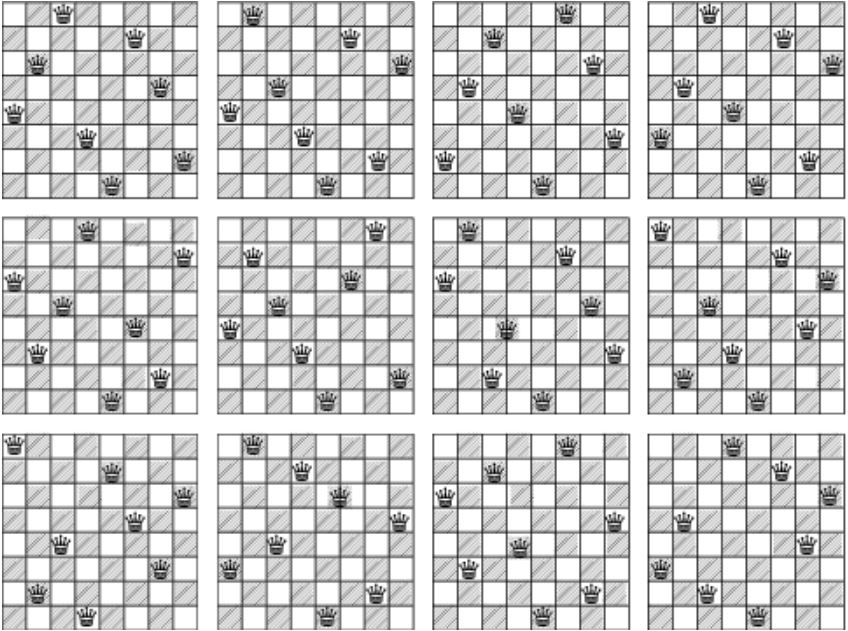
\includegraphics[scale = .25]{queen.jpg}}\\
5.0 How many (non-unique)solutions are there for $N = \{1,2,3,4,5,6\}$\\\\\\\\
5.1 What are the subproblems to the global problem of computing all possible solutions to this problem?\\\\\\\\\\
5.2 What are the possible guesses to the solutions to this problem?\\\\\\\\\\
5.3 Using 5.1 and 5.2 can you come up with a recurrence that relates subproblem solutions?\\\\\\\\
5.4 Do your subproblems follow some order that is valid?
\newpage
\noindent 6. Do not attempt this page until you put a 
lot of thought and care into problem 5. Please write
some code that attempts to produce a solution to the
N-Queen problem.
 I understand that solving problems like this on the 
 fly can be difficult. I know when I was in seminar 
 I found it to be difficult. Writing code on paper sucks.
  Try your best, I believe in you. Please come up with your
  own solution. There are many, many ways to solve this,
  and I want your attempt, not the internets.
\newpage
\noindent 4. Robert Sapolsky is a famous neuroendocrinologist (big word that means he studies hormones \& stress in humans and primates) and he's one of my favourite thinkers. He likes to use this sequence of numbers, $4, 14, 23, 34, \dots$ in his neuroscience class to illustrate an important point in categorical thinking. For purposes of our algorithms course I will call these numbers ``Sapolsky Numbers". Please compute the 10th Sapolsky Number. Can you come up with a recurrence formula for the Sapolsky numbers? (If you get stuck ask me questions)\\\\\\\\\\\\\\\\\\\\\\\\\\\\\\\\\\\\\\\\
Why was this hard? If you think you came up with a solution please tell me. 
\end{document}